\documentclass[tikz,border=8pt]{standalone}
% Shared look for every TikZ diagram. Load with \input{../../tools/tikz-style.tex}
\usepackage[T1]{fontenc}
\usepackage{lmodern}
\renewcommand{\sfdefault}{lmr}  % diagrams use the same serif as the text
\usetikzlibrary{arrows.meta, positioning, shapes.geometric, calc, fit, backgrounds}
\definecolor{cblue}{HTML}{4C78A8}
\definecolor{corange}{HTML}{F58518}
\definecolor{cgreen}{HTML}{54A24B}
\definecolor{cred}{HTML}{E45756}
\definecolor{cpurple}{HTML}{B279A2}
\definecolor{cgrey}{HTML}{6B6B6B}
\tikzset{
  every picture/.style={font=\sffamily, line width=1.2pt},
  box/.style={draw=#1, fill=#1!12, rounded corners=4pt, align=center, inner sep=7pt, minimum height=1.1cm},
  box/.default=cgrey,
  arrow/.style={-{Stealth[length=3mm]}, draw=cgrey, line width=1.4pt},
  title/.style={font=\sffamily\bfseries\Large},
  note/.style={font=\sffamily\small, text=cgrey, align=center},
}
\AtBeginDocument{\hyphenpenalty=10000 \exhyphenpenalty=10000}

\begin{document}
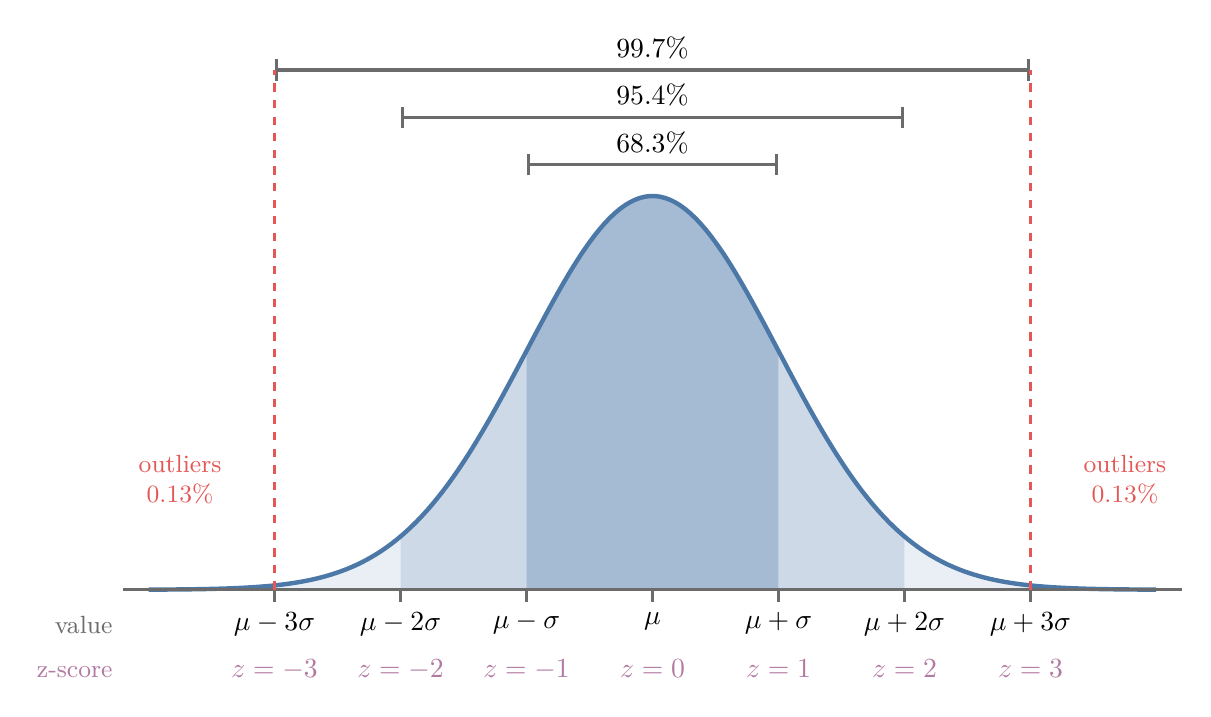
\begin{tikzpicture}[xscale=1.6, yscale=1.0]
  \def\f#1{5*exp(-(#1)*(#1)/2)}
  % bands: 3, 2, 1 standard deviations
  \fill[cblue!12] plot[domain=-3:3, samples=120] (\x,{\f{\x}}) -- (3,0) -- (-3,0) -- cycle;
  \fill[cblue!28] plot[domain=-2:2, samples=120] (\x,{\f{\x}}) -- (2,0) -- (-2,0) -- cycle;
  \fill[cblue!50] plot[domain=-1:1, samples=120] (\x,{\f{\x}}) -- (1,0) -- (-1,0) -- cycle;
  % outlier tails
  \fill[cred!60] plot[domain=3:4, samples=40] (\x,{\f{\x}}) -- (4,0) -- (3,0) -- cycle;
  \fill[cred!60] plot[domain=-4:-3, samples=40] (\x,{\f{\x}}) -- (-3,0) -- (-4,0) -- cycle;
  \draw[cblue, line width=1.6pt] plot[domain=-4:4, samples=200] (\x,{\f{\x}});
  \draw[cgrey] (-4.2,0) -- (4.2,0);
  % ticks: data scale and z scale
  \foreach \k/\lab in {-3/{\mu-3\sigma},-2/{\mu-2\sigma},-1/{\mu-\sigma},0/{\mu},1/{\mu+\sigma},2/{\mu+2\sigma},3/{\mu+3\sigma}} {
    \draw[cgrey] (\k,0) -- (\k,-0.15);
    \node[below] at (\k,-0.15) {$\lab$};
    \node[below, text=cpurple] at (\k,-0.75) {$z=\k$};
  }
  \node[left, note] at (-4.2,-0.45) {value};
  \node[left, note, text=cpurple] at (-4.2,-1.05) {z-score};
  % brackets with percentages
  \draw[|-|, cgrey] (-1,5.4) -- node[above, text=black] {68.3\%} (1,5.4);
  \draw[|-|, cgrey] (-2,6.0) -- node[above, text=black] {95.4\%} (2,6.0);
  \draw[|-|, cgrey] (-3,6.6) -- node[above, text=black] {99.7\%} (3,6.6);
  \foreach \k in {-3,3} \draw[cred, dashed] (\k,0) -- (\k,6.6);
  \node[text=cred, align=center, font=\sffamily\small] at (3.75,1.4) {outliers\\ 0.13\%};
  \node[text=cred, align=center, font=\sffamily\small] at (-3.75,1.4) {outliers\\ 0.13\%};
\end{tikzpicture}
\end{document}
